\section{Upstream tracking for \lhcb Run II}
\label{sec:up-track-run2}

\subsection{Motivation}

Following the improved performance achieved using \velout tracks within the tracking sequence of the \lhcb Upgrade, outlined in Sec.~\ref{sec:up-track-upgrade}, a similar strategy was developed for \lhcb Run II. This strategy involved using \velott tracks as input for the Forward tracking at the first stage of the software trigger. A new \velott algorithm for Run II~\cite{velott} was created based on the \velout algorithm, taking into account the slight differences in geometry between the two detectors. In the following chapter, the improved performance of the \velott algorithm for Run II compared to Run I will be shown along with the improved performance achieved when using \velott tracks rather than \velo tracks as input to the Forward tracking algorithm.

\subsection{Performance}

\subsubsection{VeloTT}

The track reconstruction efficiency, ghost rate and execution time of the VeloTT algorithm for Run I and Run II are shown in Table~\ref{tab:perf_velott_comp}. The track reconstruction efficiency as a function of \ptot and \pt are shown in Fig.~\ref{fig:eff_velott_comp}. The ghost rate as a function of \ptot and \pt are shown in Fig.~\ref{fig:gr_velott_comp}. The Run II implementation shows large improvements in terms of track reconstruction efficiency and execution time. The increased track reconstruction efficiency is most evident at high \ptot as the Run I implementation shows a negative trend for increasing \ptot. There is also a slight increase in the ghost rate. However, this is of lesser importance as the ghost rate can be further reduced during offline analysis. 

\begin{table}[!b]
\caption{The performances of the VeloTT algorithms for Run I and Run II in terms of track reconstruction efficiency, ghost rate and execution time.}
\label{tab:perf_velott_comp}
\begin{center}
  \begin{tabular}{c|c|c|c}
    VeloTT & Efficiency [\%] & Ghost rate [\%] & Timing [ms] \\ 
    \hline
    Run I  &  92.74  &  \hphantom{0}7.21  &  32.50  \\ 
    Run II  &  97.77  &  11.60  &  \hphantom{0}0.50   \\ 
  \end{tabular}
\end{center}
\end{table}

\begin{figure}[!tb]
\begin{center}
  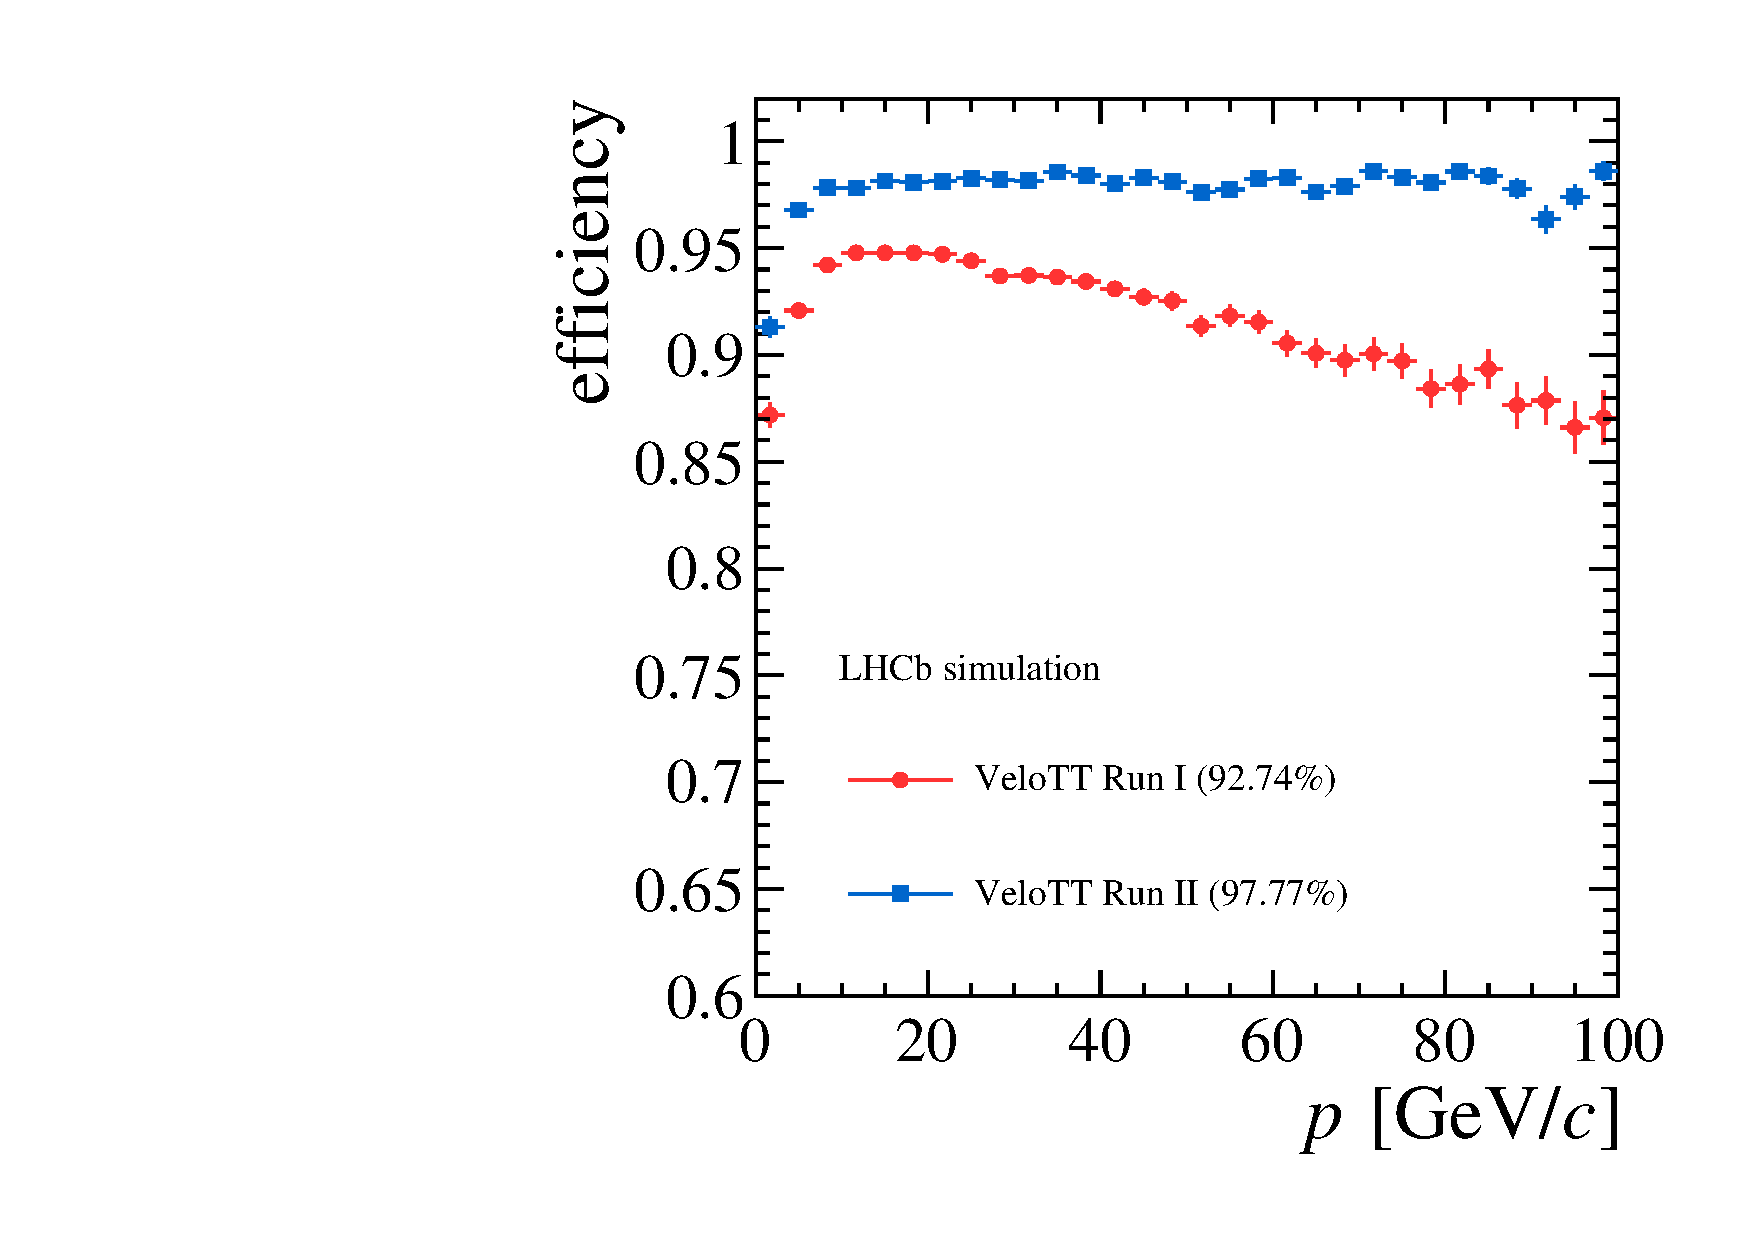
\includegraphics[width=0.45\linewidth]{figs/upstream-tracking-run2/VeloTT-eff-p.pdf}
  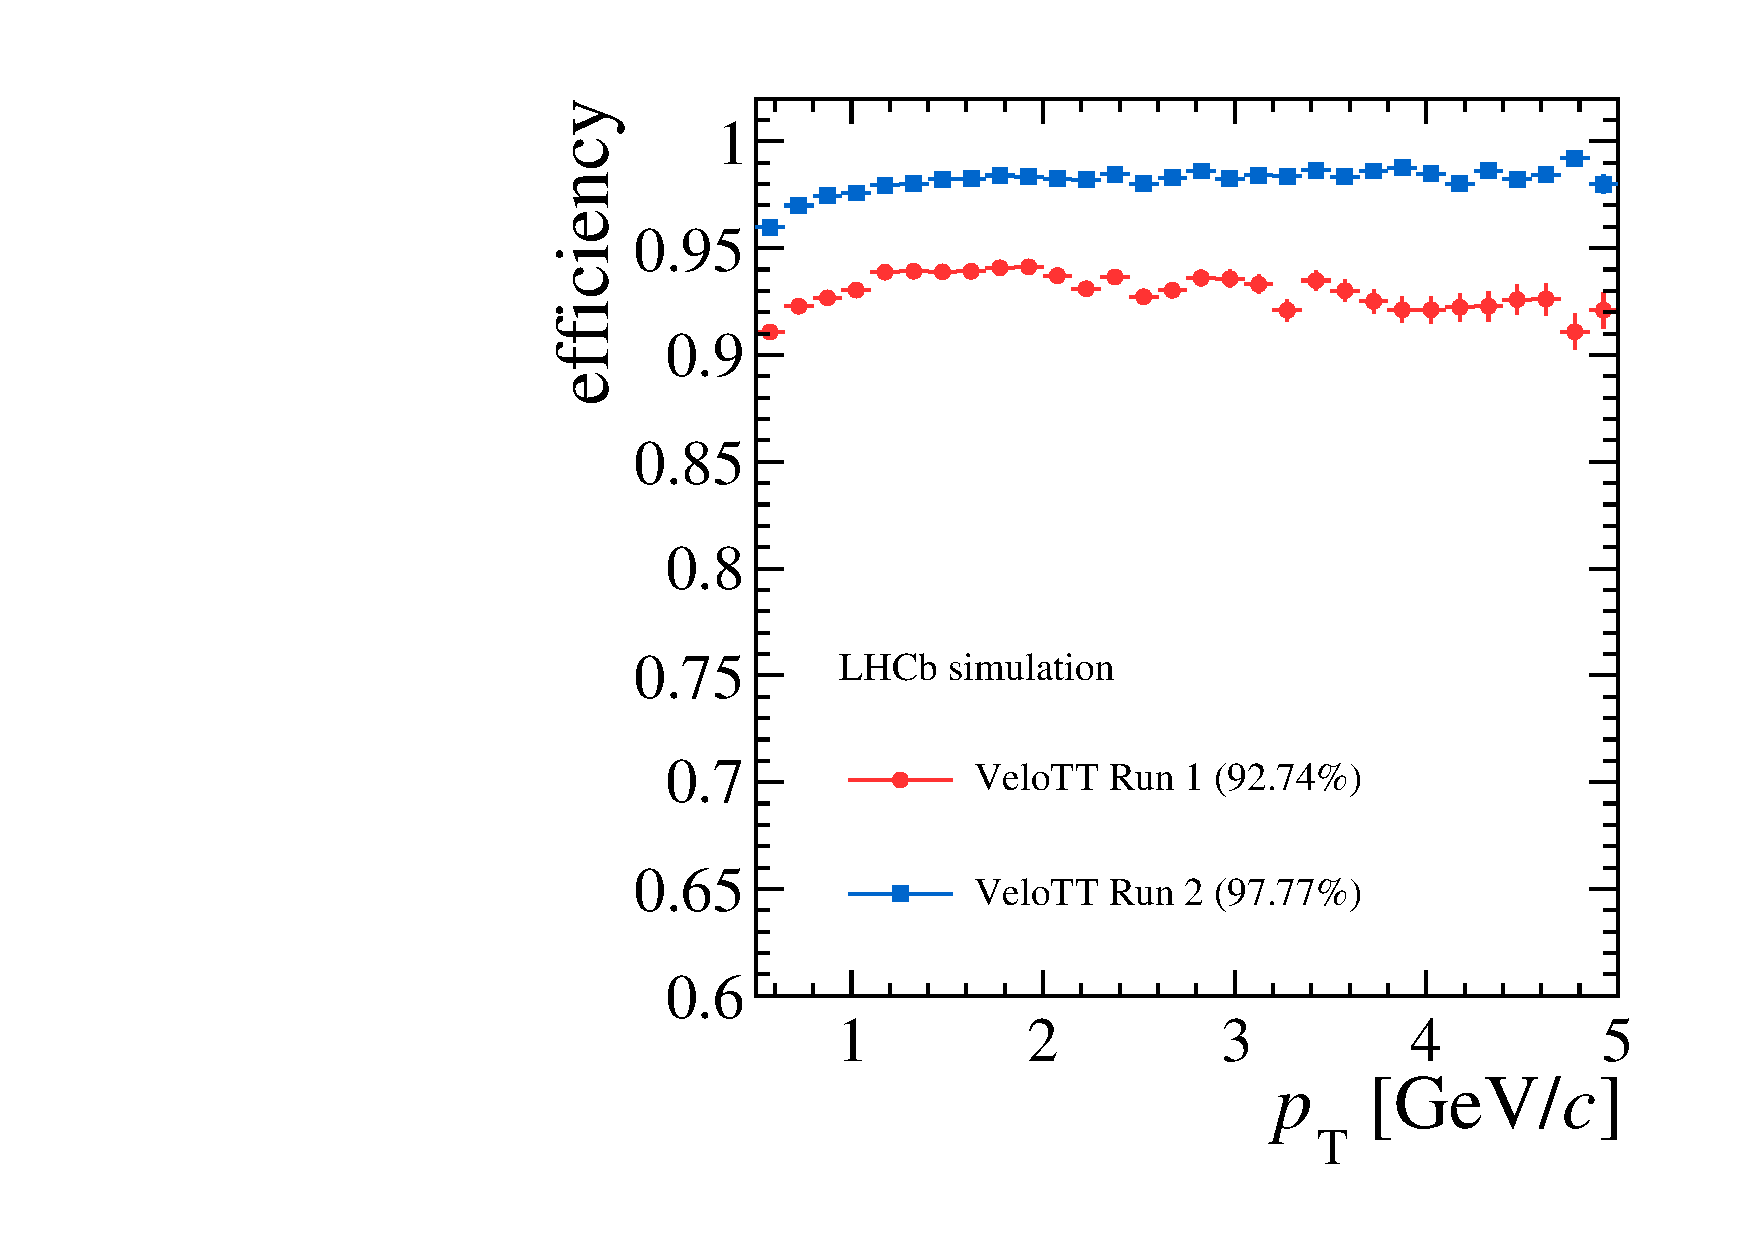
\includegraphics[width=0.45\linewidth]{figs/upstream-tracking-run2/VeloTT-eff-pt.pdf}
  \caption{The track reconstruction efficiency of the VeloTT algorithms for Run I and Run II as a function of \ptot and \pt.}
  \label{fig:eff_velott_comp}
  \end{center}
\end{figure}

\begin{figure}[!tb]
  \begin{center}
    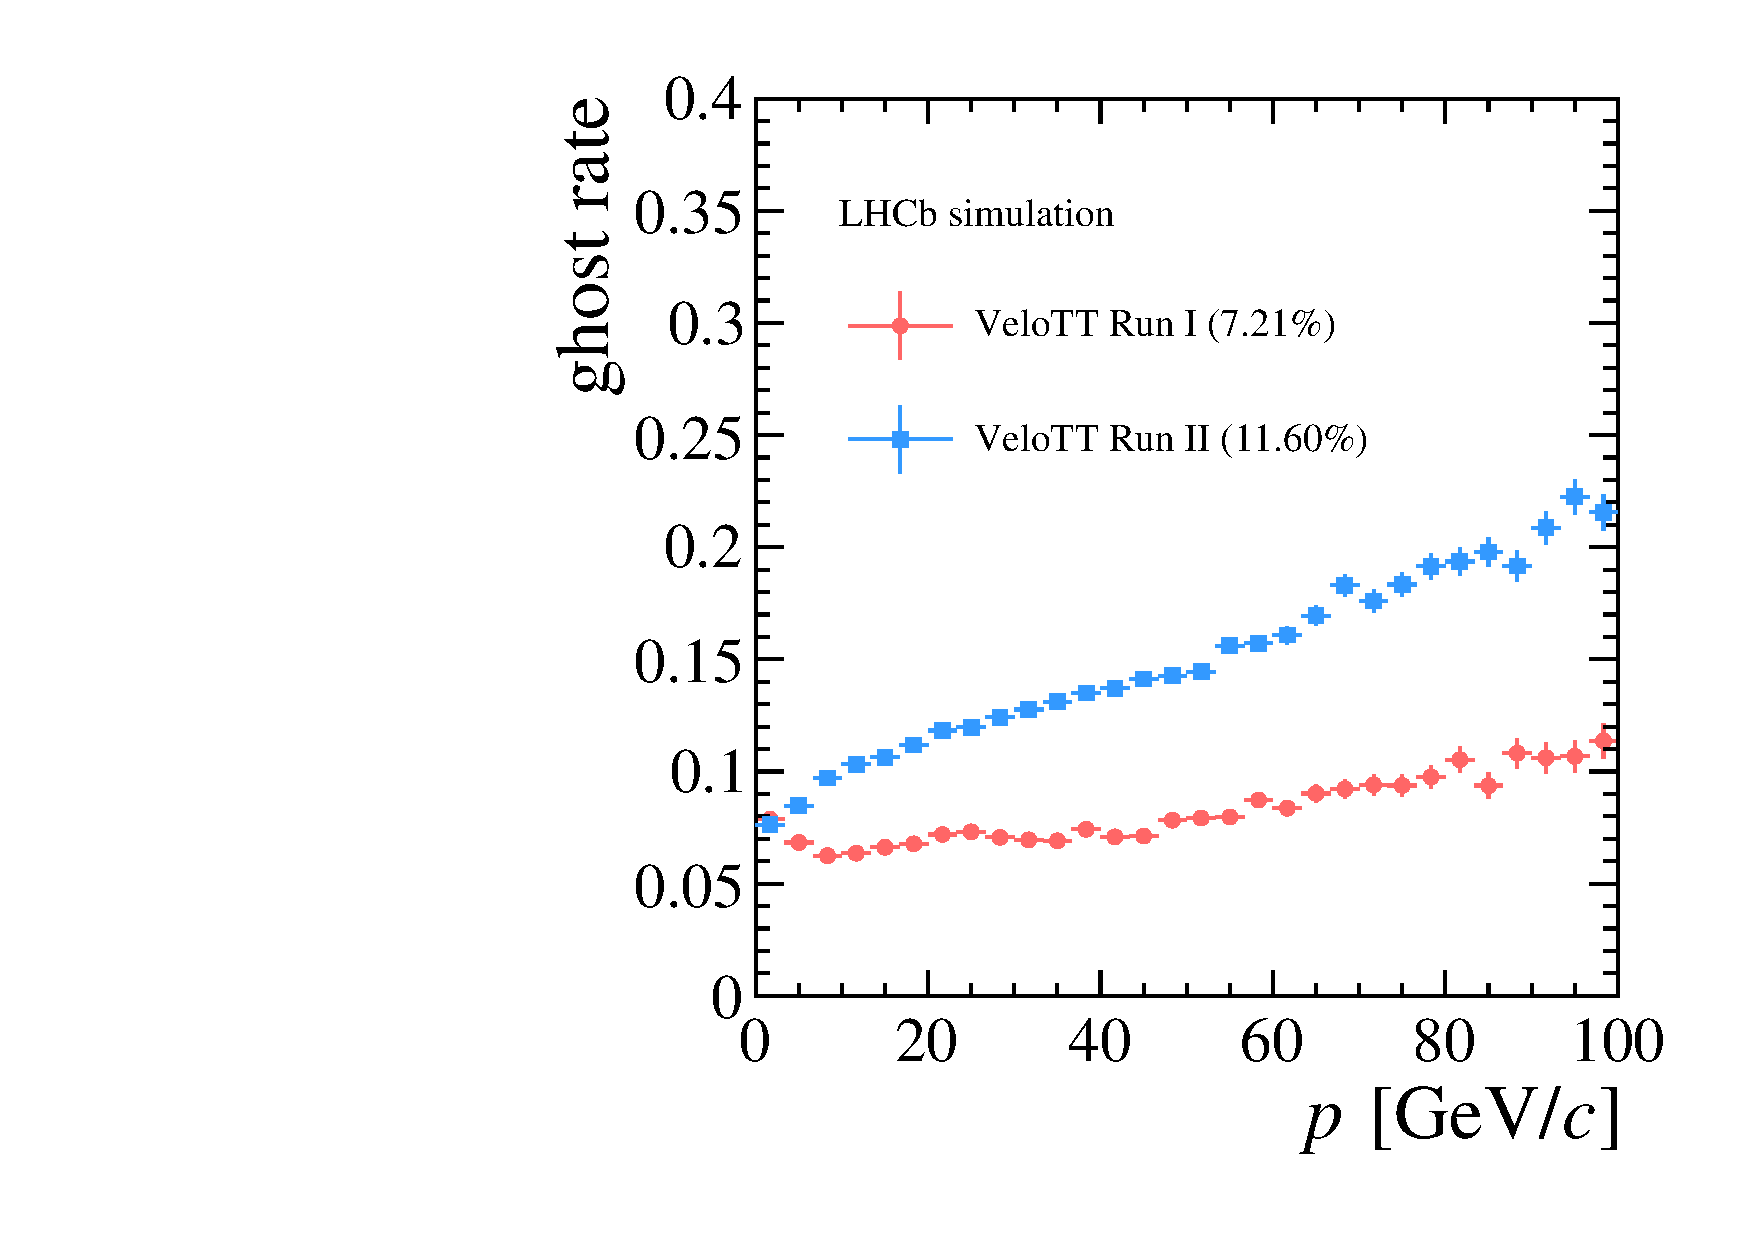
\includegraphics[width=0.45\linewidth]{figs/upstream-tracking-run2/VeloTT-gr-p.pdf}
    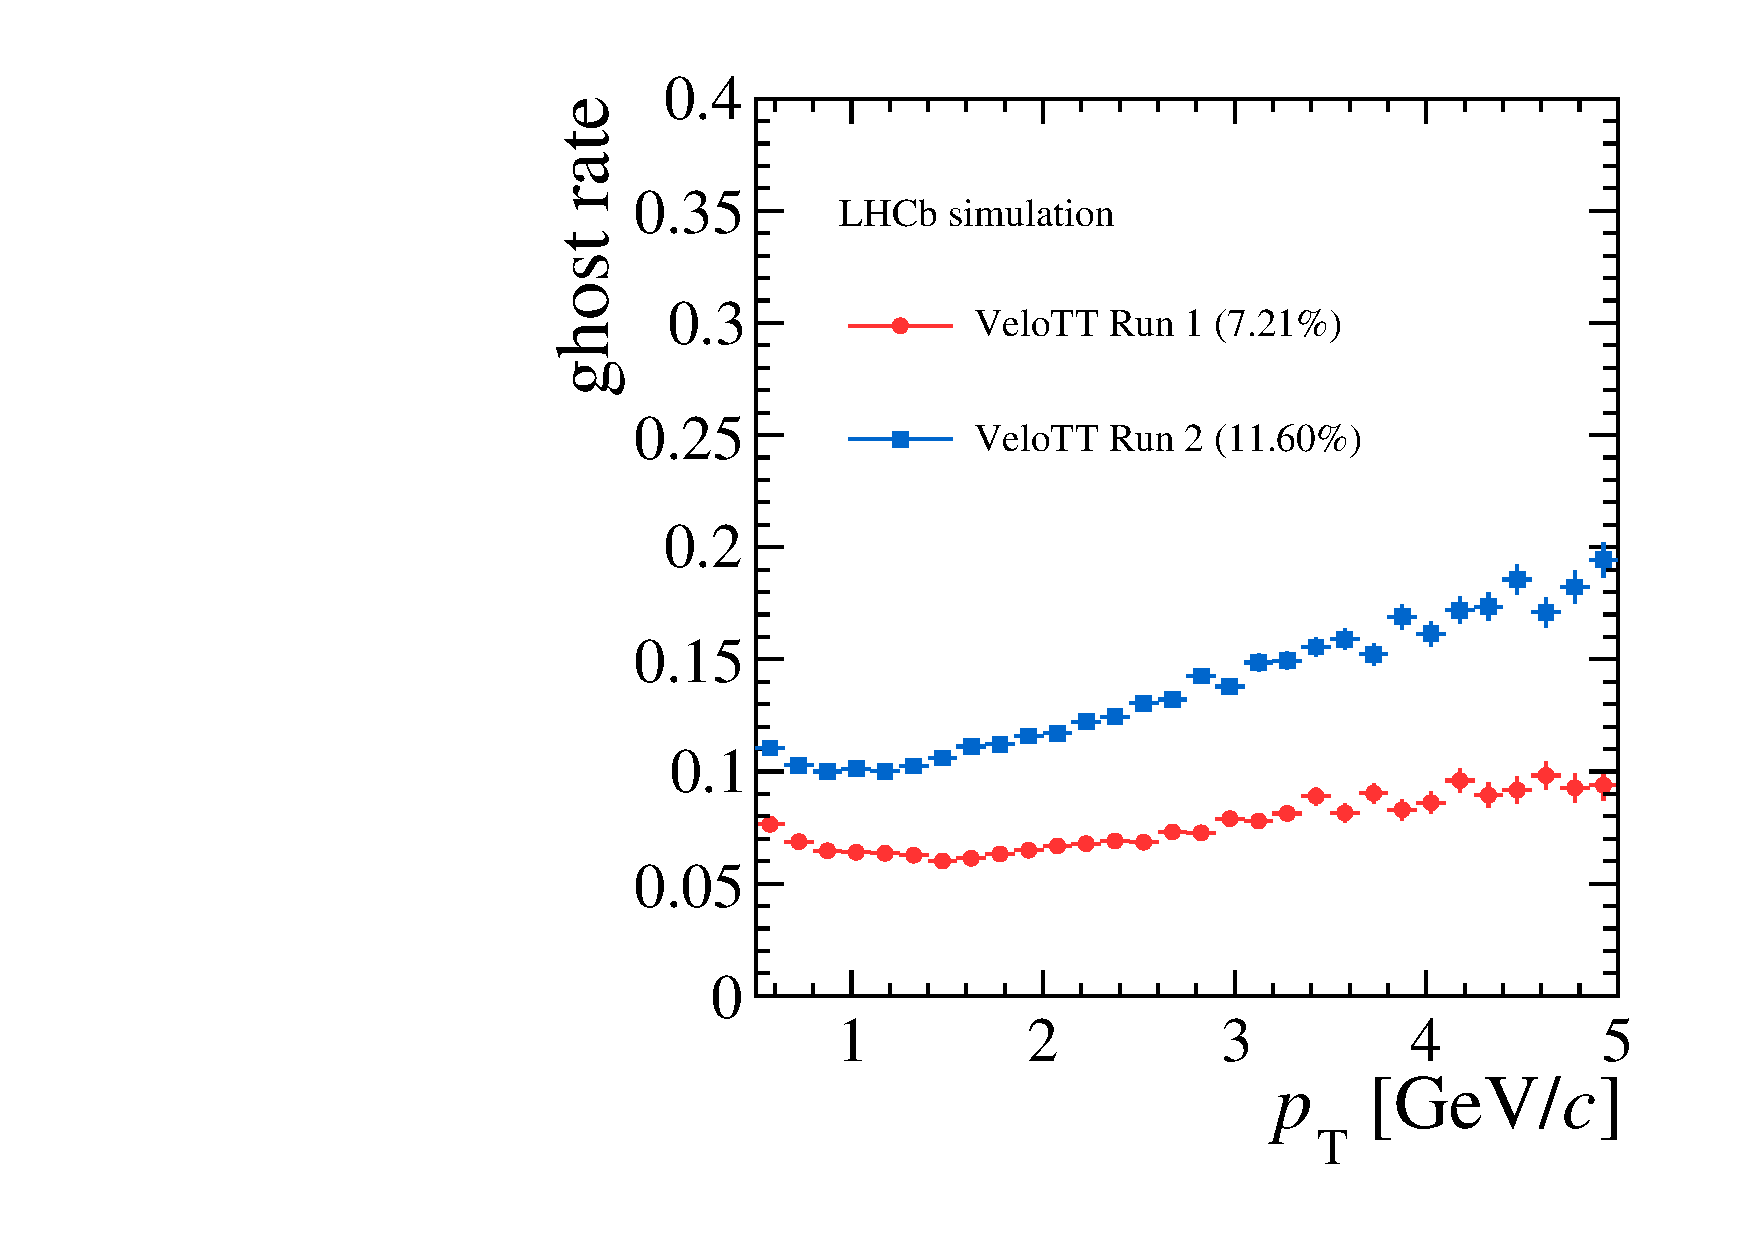
\includegraphics[width=0.45\linewidth]{figs/upstream-tracking-run2/VeloTT-gr-pt.pdf}
    \caption{The ghost rate of the VeloTT algorithms for Run I and Run II as a function of \ptot and \pt.}
    \label{fig:gr_velott_comp}
  \end{center}
\end{figure}

\subsubsection{Forward}

The track reconstruction efficiency, ghost rate and execution time of the Forward algorithm taking \velo or VeloTT tracks as input are shown in Table~\ref{tab:perf_forward_run2_comp}. The track reconstruction efficiency as a function of \ptot and \pt are shown in Fig.~\ref{fig:eff_forward_run2_comp}. The ghost rate as a function of \ptot and \pt are shown in Fig.~\ref{fig:gr_forward_run2_comp}. The use of VeloTT tracks as input drastically reduces the ghost rate and execution time of the Forward algorithm. This comes at a small cost the in track reconstruction efficiency. This efficiency is retrieved in the second stage of the software trigger~\cite{hlt-runII}.

\begin{table}[!tb]
  \caption{The performances of the Forward algorithm using \velo or VeloTT tracks as input in terms of track reconstruction efficiency, ghost rate and execution time.}
  \label{tab:perf_forward_run2_comp}
  \begin{center}
    \begin{tabular}{c|c|c|c|c}
      & Efficiency [\%] & Ghost rate [\%] & VeloTT [ms] & Forward [ms] \\ 
      \hline
      Velo-Forward  & 93.15  & 46.86  &  -  & 13.71 \\ 
      VeloTT-Forward  & 89.23  & 17.13  &  0.50 & \hphantom{0}4.08 \\
    \end{tabular}
  \end{center}
\end{table}

\begin{figure}[!tb]
  \begin{center}
    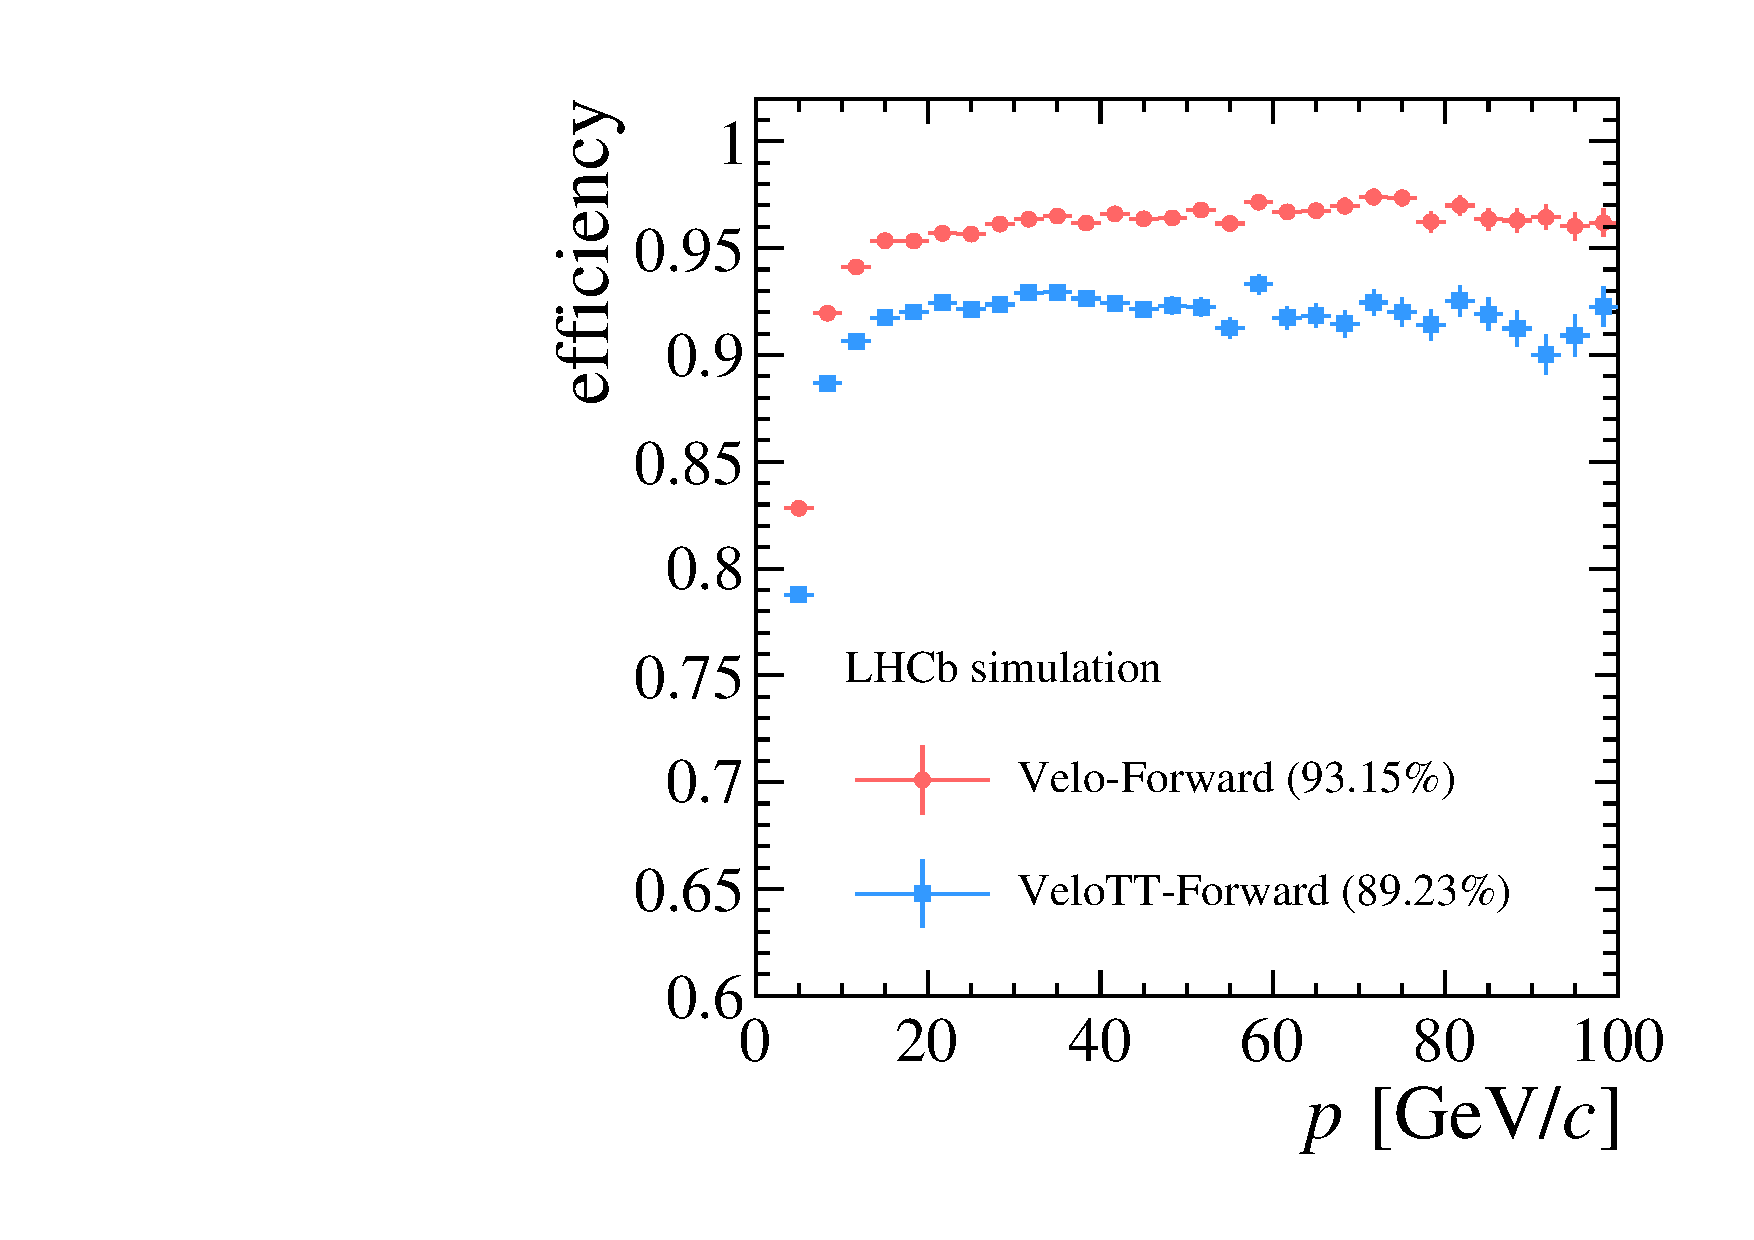
\includegraphics[width=0.45\linewidth]{figs/upstream-tracking-run2/Forward-eff-p.pdf}
    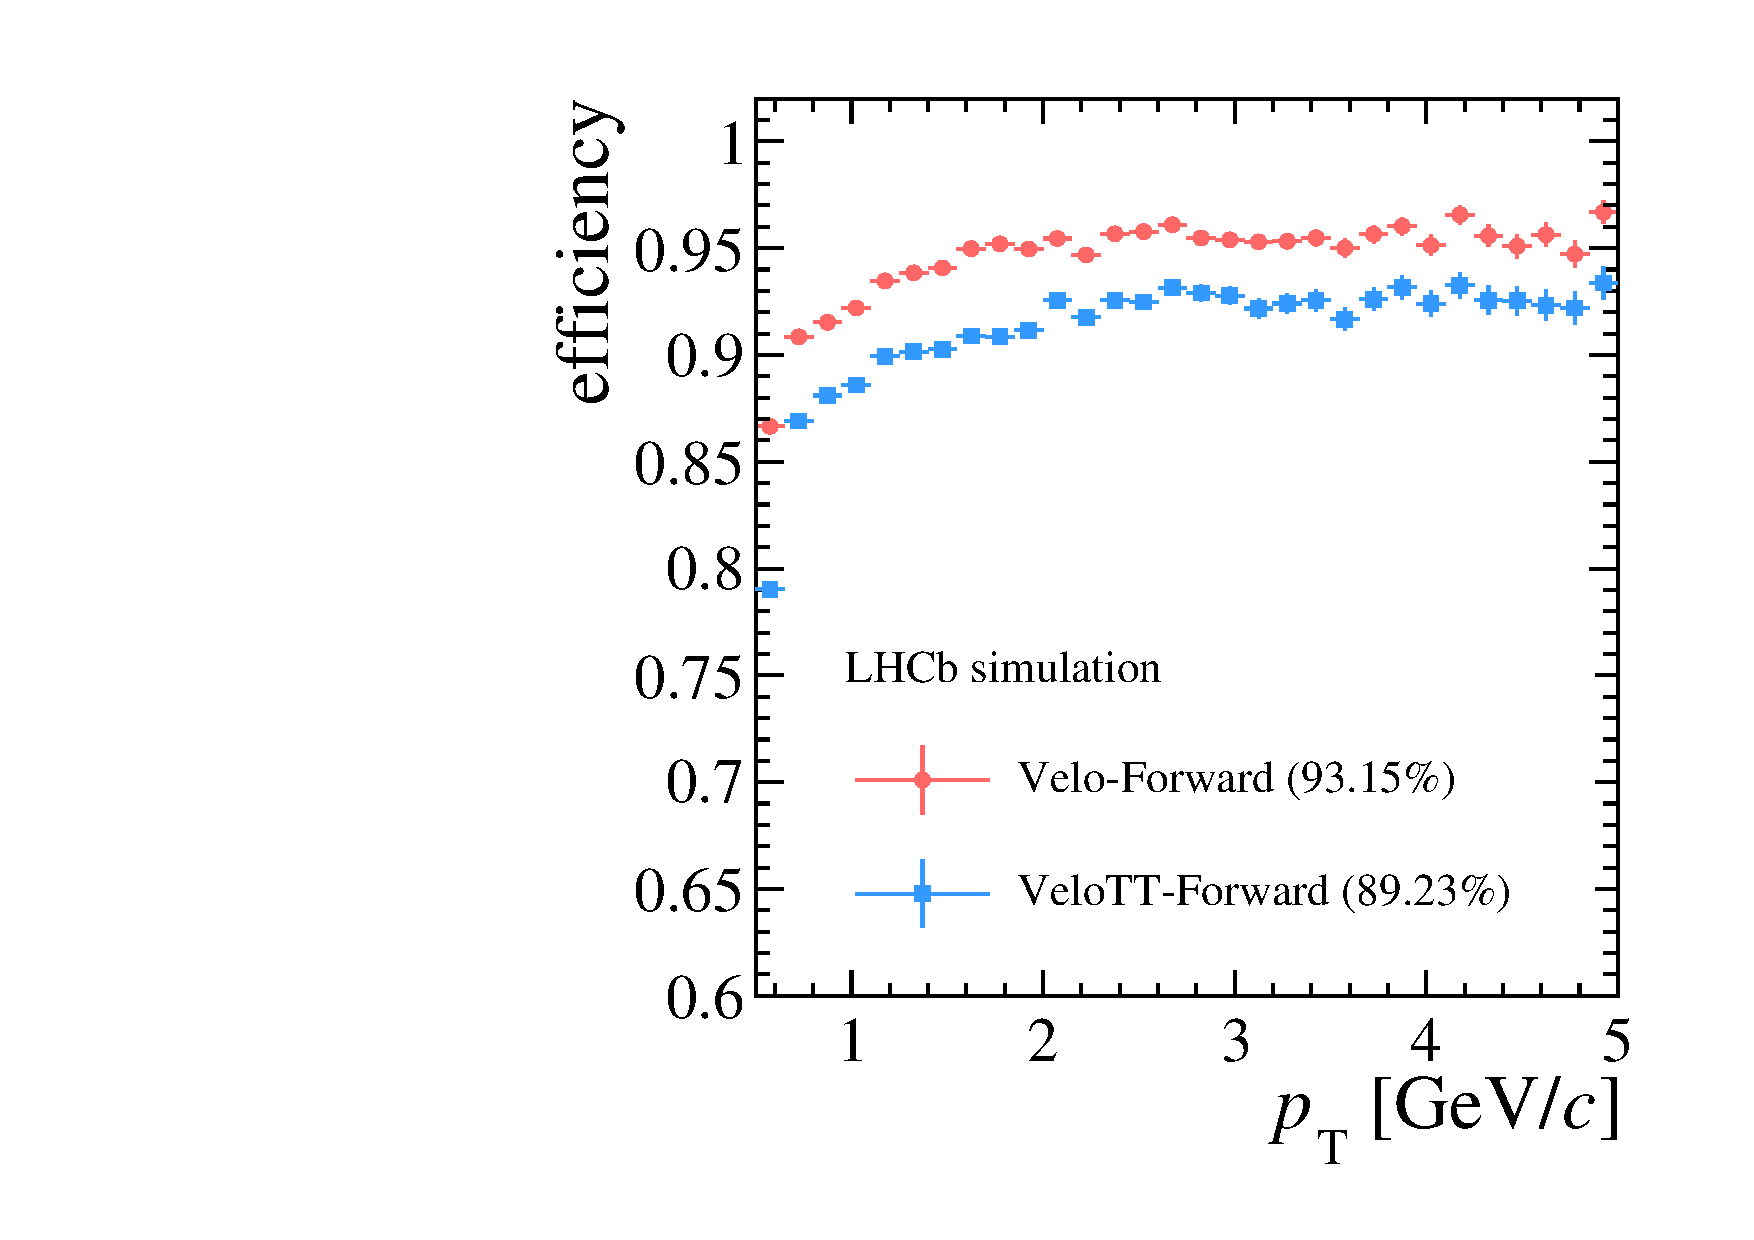
\includegraphics[width=0.45\linewidth]{figs/upstream-tracking-run2/Forward-eff-pt.pdf}
    \caption{The track reconstruction efficiency of the Forward algorithm using \velo or VeloTT tracks as a function of \ptot and \pt.}
    \label{fig:eff_forward_run2_comp}
  \end{center}
\end{figure}

\begin{figure}[!tb]
  \begin{center}
    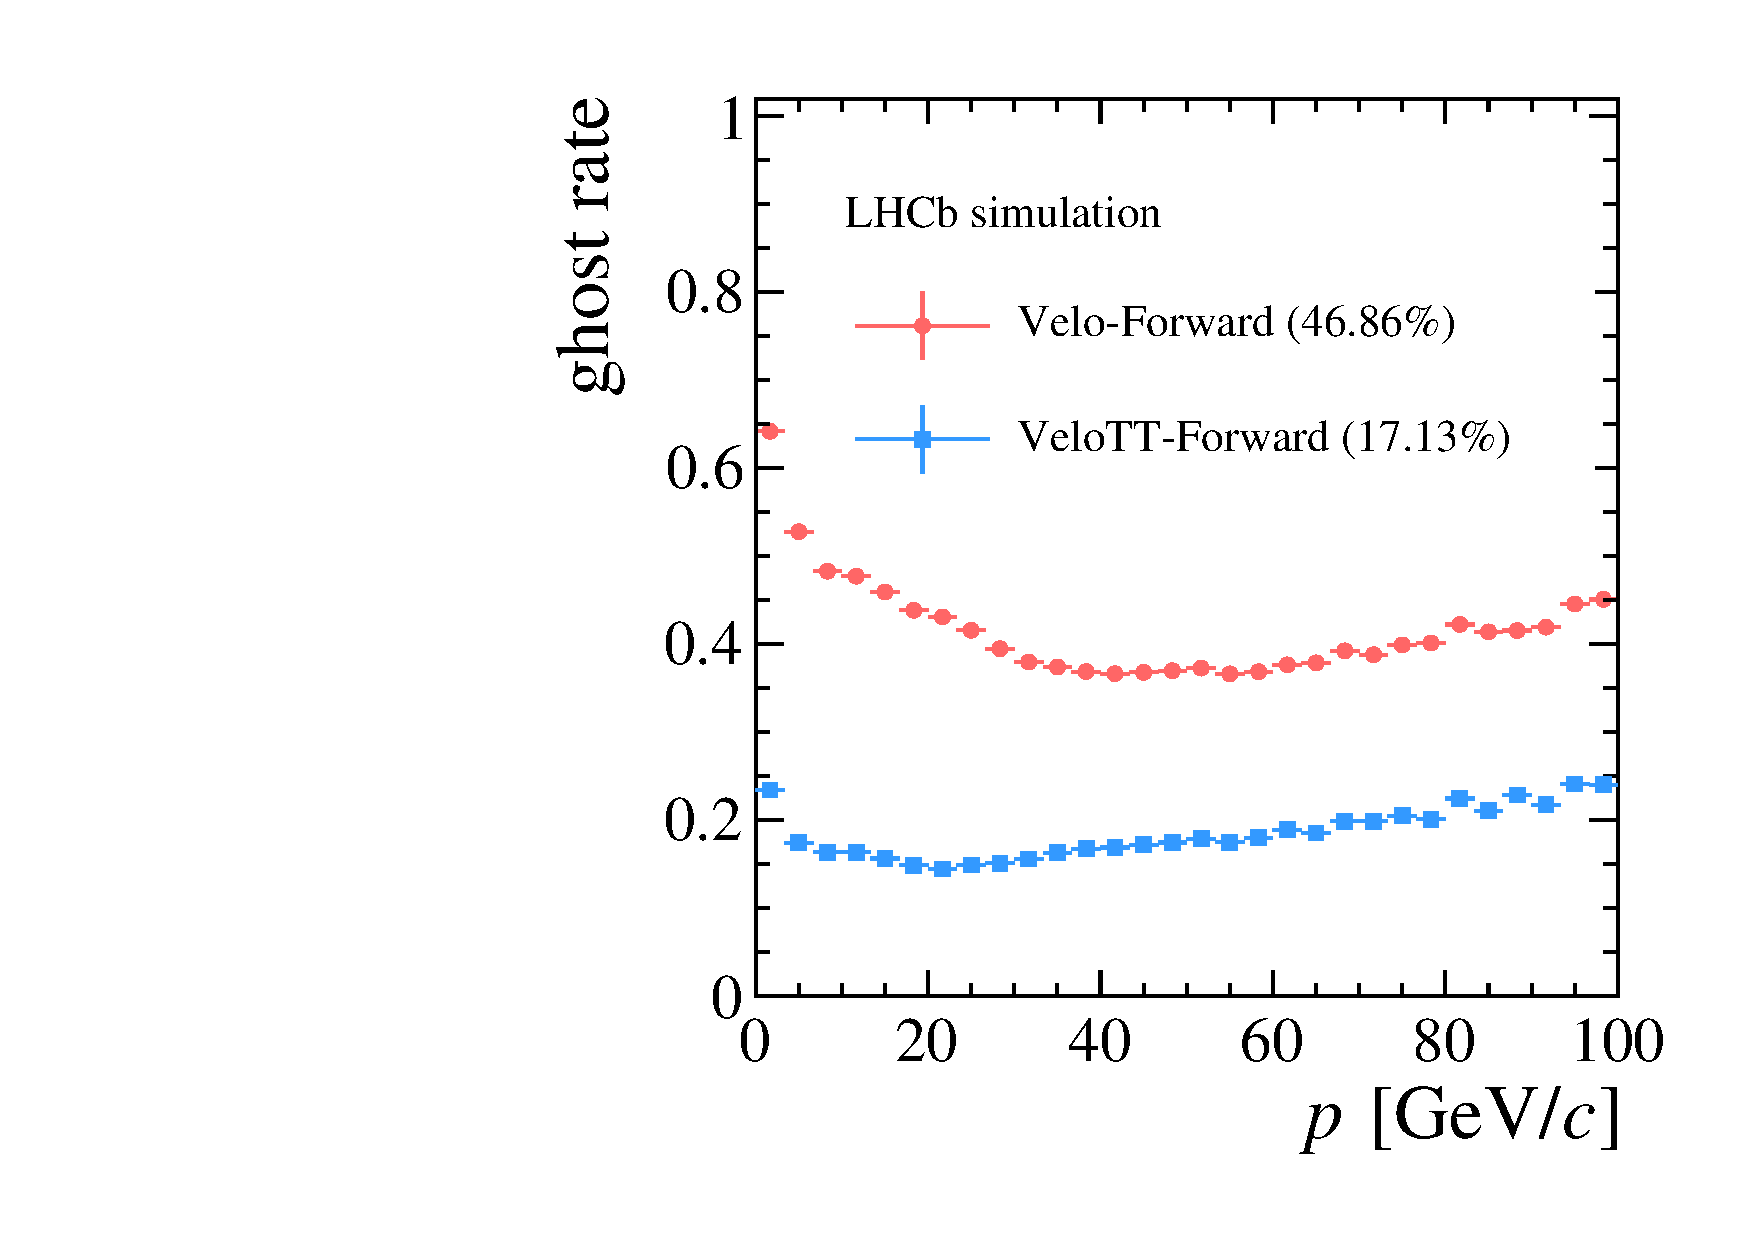
\includegraphics[width=0.45\linewidth]{figs/upstream-tracking-run2/Forward-gr-p.pdf}
    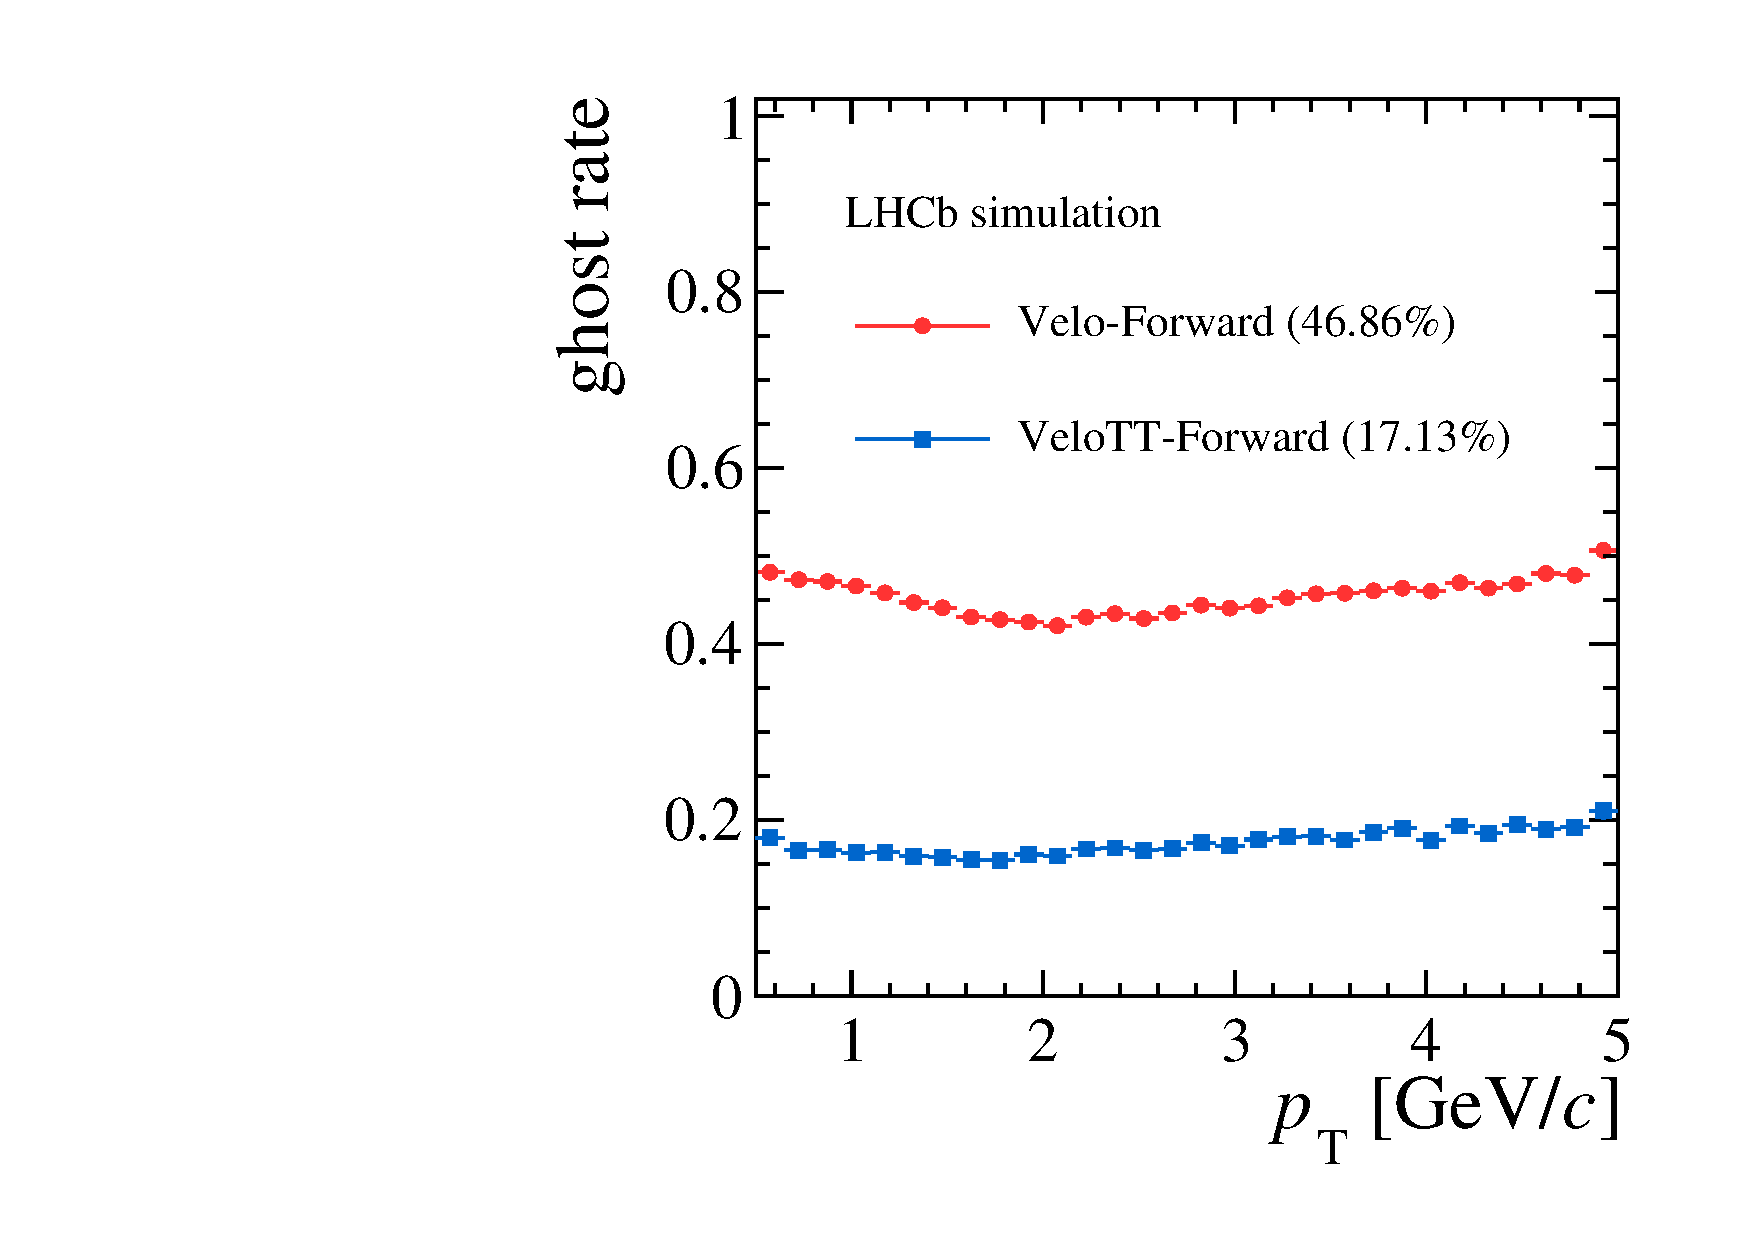
\includegraphics[width=0.45\linewidth]{figs/upstream-tracking-run2/Forward-gr-pt.pdf}
    \caption{The ghost rate of the Forward algorithm using Velo or VeloTT tracks as a function of \ptot and \pt.}
    \label{fig:gr_forward_run2_comp}
  \end{center}
\end{figure}

\subsection{Summary}
\label{sec:up-track-run2:summary}

The enhanced performance obtained by introducing the VeloTT algorithm into the reconstruction chain in Run II resulted in two important improvements. Firstly, it is possible to remove any IP requirement on \velo tracks and to loosen the \pt threshold of the Forward tracking from 1.2\gevc to 0.5\gevc in the first stage of the software trigger. This greatly improves the signal efficiency for charm physics and allows lifetime unbiased triggers for hadronic final states for the first time~\cite{hlt-runII}. Secondly, significant improvements to the reconstruction sequence in the second stage of the software trigger have allowed the convergence of the online and offline reconstruction. Combined with a novel approach providing real-time alignment and calibration~\cite{alignment}, this allows physics analyses to be performed directly on the output of the software trigger~\cite{turbo}. Only writing out the information of the signal candidates leads to a large saving in storage space ($\sim 90$\%). This is ideal for the analysis of channels with high yields that would previously have been heavily pre-scaled. It also allows rapid turn-around from data taking to analysis on the order of a few weeks~\cite{jpsi-em,charm-em}.
